\newpage
\section{Optimization models review}

% Scheduling
\subsection{Scheduling}

Nell'ambito dei problemi dello scheduling abbiamo degli elementi ben specificati:

\begin{itemize}
	\item \hl{task/job} già assegnati
	\item $n$ \hl{macchine/processori}
	\item potremmo attrezzare le macchine con dei \hl{tools}
\end{itemize}

Intendiamo \hl{allocare i tasks alla macchine in "overtime"} quindi capire anche la \hl{fascia temporale nella quale eseguire il task}. Potrebbe esserci un unico tempo di esecuzione oppure un task può avere dei tempi di esecuzione differenti su macchine differenti. 

L'output sarà un diagramma di Ganth.

\hl{I task possono avere degli istanti di rilascio} dove non potrebbe essere rilasciato dopo un certo istante di tempo (\hl{ready time}).

Possono esserci delle \hl{relazioni di precedenza tra i tasks}. Quindi non posso effettuare un task se prima non ho concluso l'altro.

Il diagramma mi dice nel tempo a che macchina è associato quale task ed in quali intervalli di tempo e con quale tool.


% Project scheduling
\subsection{Project scheduling}

Per progetto intendiamo un \hl{insieme di tasks che sono realizzati al fine di raggiungere un goal}. La caratteristica di un progetto è che nel complesso le attività non sono mai state eseguite in precedenza.

Le \hl{caratteristiche di un progetto} sono:


\begin{itemize}
	\item \textbf{durata delle attività} che nota
	\item ha \textbf{a capo un Project Manager}: responsabile del progetto e dei tempi di realizzazione, costi di produzione, ecc...
\end{itemize}

Un progetto è \hl{rappresentato da diverse attivita'} in una tabella fornita dal Project Manager:


\begin{table}[h!]
	\begin{center}
	\begin{tabular}{|c | c c |} 
		\hline
		Attività & Durata stimata $d_i$ & Predecessori \\ [0.5ex]
		\hline
 		1 & 10 & - \\
		2 & 10 & - \\
		3 & 10 & 1 \\
		4 & 10 & 1, 2 \\
		\hline
		\end{tabular}
	\end{center}
	\caption{Tabella di ore di lavoro e predecessioni delle attività}
	\label{tabatt}
\end{table}


e in un diagramma aciclico (Activity On Node (AoN)):


\begin{figure}[H]
\centering
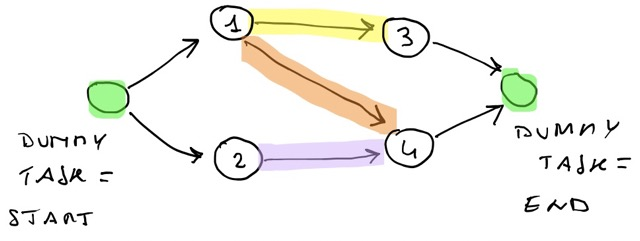
\includegraphics[scale=0.4]{aon.jpeg}
\caption{Diagramma Activity On Node} 
\label{aon}
\end{figure}


dove abbiamo degli "archi" che rappresentano le predecessioni. Avremo anche dei \hl{vertici fittizzi}:

\begin{itemize}
	\item start: lo colleghiamo tutte le attività che non hanno predecessori
	\item end: ci colleghiamo tutte le attività finali
\end{itemize}

Una funzione fondamentale del Project Manager è la possibilità di accelerare alcune attività agendo su:

\begin{itemize}
	\item \hl{Variabili decisionali}:
		
		nel nostro caso, è lo \hl{start time $s_i$}. Ipotizziamo che il progetto inizi al tempo $t = 0$, quindi per ogni task abbiamo che:

			$$s_i \geq 0\ \ \ \forall\ \ \ i \in TASKS$$

		In più possiamo definire \hl{$T \geq 0$ tempo di completamento del progetto} (\textbf{completion time}).

		Minimizziamo il completion time:

			$$\min z = T$$

		con $z = 1T + 0s_1 + 0s_2 + ... + 0s_n$
		
		
	\item \hl{relazioni di precedenza}:
	
		relazioni che portano alcuni nodi a dipendere da altri:
		
		$$
		p_{ij}=
		\begin{cases} 
		    1 \Leftrightarrow i \in j \\ 
		    0 altrimenti
		\end{cases}$$
		
		con \hl{$p_{ij}$ matrice} costate e binaria:
		
		$$p =
		\left[ {\begin{array}{cccc}
		    0 & 0 & 1 & 1 \\
			0 & 0 & 0 & 1 \\
		    0 & 0 & 0 & 0 \\
		    0 & 0 & 0 & 0 \\
		\end{array} } \right]$$
		
	
	\item \hl{vincoli di precedenza}:
	
		Sia \hl{$T$ maggiorante del tempo di completamento delle task}:
			$$s_i + d_i \leq T$$

		allora:

			$$p_{ij} (s_i + d_i) \leq s_j\ \ \ \forall\ \ \ i,j \in TASKS$$

		Possiamo avere che:

		\begin{itemize}
			\item \hl{$p_{ij} = 1$}: allora \textbf{$i$ è predecessore di $j$} quindi il tempo di inizio del task $j$ deve essere successivo o uguale al task $i$ cioè $s_i + d_i$
	
			\item \hl{$p_ij = 0$}: $i$ non è predecessore quindi avremo $0 \leq s_j$ allora il vincolo è ridondante
		\end{itemize}
		
		scriviamo allora:
 
		$$s_i + d_i \leq s_j\ \ \ \forall\ \ \ i,j \in TASKS,\ p_{ij} \geq 0$$


\end{itemize}


% Esempio
\subsection{Esempio }

Un modello espanso per problemi di istanza:

\begin{enumerate}
	\item funzione obiettivo: $\min z = T$
	\item vincoli:
		\begin{itemize}
			\item $s_1 + 10 \leq T$
			\item $s_2 + 10 \leq T$
			\item $s_3 + 10 \leq T$
			\item $s_4 + 10 \leq T$
			\item $s_1 + 10 \leq s_3 (p_{13} = 1)$
			\item $s_1 + 10 \leq s_4 (p_{14} = 1)$
			\item $s_2 + 10 \leq s_4 (p_{24} = 1)$
			\item $s_1, s_2, s_3, s_4 \geq 0$
			\item $T \geq 0$
		\end{itemize}
\end{enumerate}


% Velocizzazione del progetto
\subsection{Velocizzazione del progetto}

Il Project Manager ha un \hl{budget} per poter velocizzare il progetto.

Se considero un \hl{task $i$ con durata non costante ($d_i^N$)}, avremo un valore nominale che dipende da un budget extra.

Il più semplice è l'\hl{andamento lineare} dove all'aumentare delle risorse la durata si riduce in modo lineare. Il che è vero finché non si incontra un \hl{vincolo inferiore $d_i^m$}.


Le \hl{3 risorse} alle quali si possono far riferimento sono le \hl{3M}:

\begin{itemize}
	\item Man
	\item Machine
	\item Money
\end{itemize}


quindi $d_i = d_i^N$.


\begin{figure}[H]
\centering
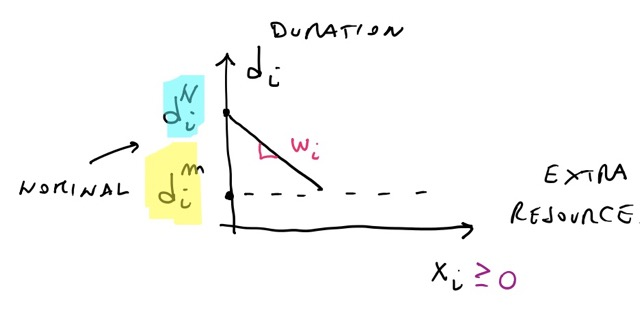
\includegraphics[scale=0.4]{budget.jpeg}
\caption{Diagramma budget} 
\label{budget}
\end{figure}


con:

\begin{itemize}
	\item \hl{pendenza w}: \textbf{riduzione della durata del task $i$} per unità di extra risorse (mesi di lavoro / k euro)
	\item $d_i = d_i^N - w_i x_i \geq d_i^m$ vincolo del valore minimo per task
	\item $x_i$: denaro usato per il task $i$
	\item $B$: budget totale

\end{itemize}


% Esempio velocizzazione progetto
\subsection{Esempio velocizzazione progetto}

Avremo un modello con:

\begin{enumerate}
	\item funzione obiettivo: $\min z = T$
	\item vincoli:
		
		\begin{itemize}
			\item $s_i + d_i^N - w_i x_i \leq T\ \ \ \forall\ \ \ i \in TASKS$
			\item $s_i + d_i^N - w_i x_i \leq s_j\ \ \ \forall\ \ \ i, j \in TASKS, p_{ij} = 1$
			\item $d_i^N - w_i x_i \geq d_i^m\ \ \ \forall\ \ \ i \in TASKS$
			\item $\sum_{i \in TASKS} x_i \leq B$
			\item $T \geq 0$
			\item $s_i \geq 0\ \ \ \forall\ \ \ i \in TASKS$
			\item $x_i \geq 0\ \ \ \forall\ \ \ i \in TASKS$
		\end{itemize}
\end{enumerate}


% Low sizing models
\subsection{Low sizing models}

Sono in genere usati da aziende manifatturiere. 


\begin{figure}[H]
\centering

\includegraphics[scale=0.3]{prodline.jpeg}
\caption{Processo produtivo} 
\label{procprod}
\end{figure}


Supponendo di avere un \hl{tasso di domanda $d$} costante in base al tipo di prodotto. Ogni tipo di prodotto si differenzia dagli altri con una piccola modifica come può essere un differente gusto per una produzione di yogurt.

Questa differenziazione porta ad un \hl{costo di setup} delle macchine che andranno pulite, generando un costo fisso $k$.

Il livello di scorte sarà rappresentato con dei picchi con ampiezza $q$:


\begin{figure}[H]
\centering
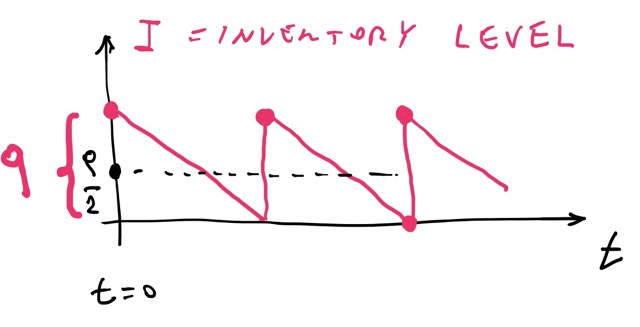
\includegraphics[scale=0.3]{invlev.jpeg}
\caption{Livello di inventario} 
\label{invlev}
\end{figure}


avendo una domanda costante, avremo una diminuzione lineare nello scorte di magazzino.

Ovviamente avremo dei \hl{costi medi di stockaggio $h$} dato che le scorte si "muoveranno" scambiandosi con altre scorte che entrano nel magazzino. Quindi andremo a calcolare il costo in base alla giacenza del \hl{numero di scorte medie $\frac{q}{2}$}.

In base alla strategia avremo:

\begin{enumerate}
	\item \hl{caso estermo}:
	
		gestione di tipo \textbf{just in time} dove \textbf{produco solo sotto commissione del cliente}.

		Avremo quindi:
		
		\begin{itemize}
			\item \textbf{livello di scorte molto basso} con un livello medio delle scorte molto basso e dei \textbf{costi di stockaggio bassi}
			\item \textbf{maggioramento dei costi del setup}
			\item pago $k$ più volte durante l'anno
		\end{itemize}
		
	\item \hl{caso produzione annua}:
	
		si produce un \textbf{quantitativo pari alla domanda annua}.
		
		Avremo quindi:
		
		\begin{itemize}
			\item grandi \textbf{costi di stockaggio}
			\item pago $k$ solo una volta all'anno
		\end{itemize}

\end{enumerate}


\begin{figure}[H]
\centering
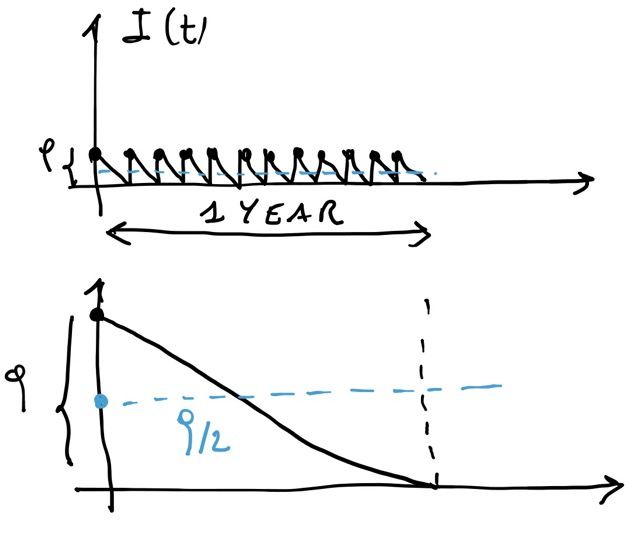
\includegraphics[scale=0.3]{casipart.jpeg}
\caption{Casi particolari} 
\label{casipart}
\end{figure}


% Scrivere il modello di ottimizzazione
\subsection{Scrivere il modello di ottimizzazione}

Le fasi da seguire prevedono la scrittura di:

\begin{enumerate}
	\item \hl{variabili decisionali}: variabile matematica per descrivere la mia decisione
	\item \hl{funzione obiettivo}: costo totale annuale composto dal \textbf{costo di scorta e quello di setup}
\end{enumerate}

Avremo allora:

$$z = k \frac{d}{q} + h \frac{q}{2} $$


Per la \hl{soluzione ottima}, faccio il gradiente:

$$\frac{dz}{dq} = 0 \Leftrightarrow -k \frac{d}{q^2} + \frac{h}{2} = 0$$


Concludiamo che il \hl{lotto economico}, per minimizzare i costi, sarà raggiunto da:

$$q^* = \sqrt{\frac{2kd}{h}}$$


\begin{figure}[H]
\centering
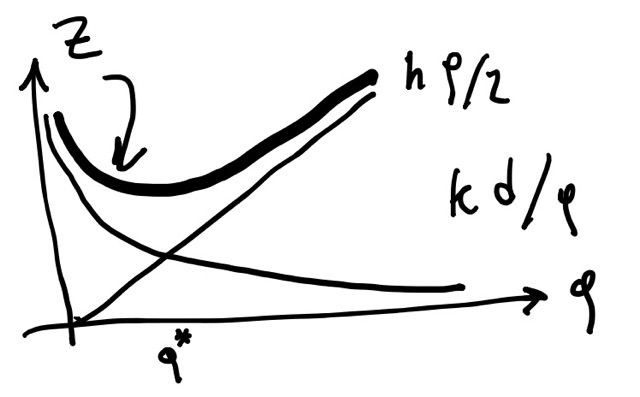
\includegraphics[scale=0.3]{lottoec.jpeg}
\caption{Caso di lotto economico} 
\label{lottoec}
\end{figure}



Questo modello \hl{nella pratica ha dei limiti} dati i possibili vincoli come:

\begin{itemize}
	\item spazio limite di un magazzino
	\item produzione di più prodotti contemporaneamente
	\item vincolo di immobilizio
	\item vincolo sul capitale
	\item ecc ...
\end{itemize}


Associati al vincolo di immobilizzo possiamo avere anche un \hl{limite nei prodotti che posso fare di A e di B}. Se si ipotizza una domanda costante, ho che il \hl{costo totale annuale $z$} sarà data dal costo annuale di A e di B:

$$z = (k_A \frac{d_A}{q_A} + h_A \frac{q_A}{2}) + (k_B \frac{d_B}{q_B} + h_B \frac{q_B}{2})$$


Avremo che $z$ è dato da 2 termini uno che dipende da A ed uno da B. Per noi supponiamo che $k_A = k_B = k$.

Di conseguenza anche i lotti di approvvigionamento possono essere diversi. Quindi, quando è necessario, avremo che dovremo \hl{decidere quante confezioni produrre di A e quante di B}.

Nel \hl{caso peggiore ipotizzo che la produzione contemporanea di 2 lotti}, quindi non dovrà superare la capacità di magazzino $Q$:

$$q_A + q_B \leq Q\ \ \ \forall\ \ \ q_A, q_B \geq 0$$

dove la produzione contemporanea indica la \hl{sovrapposizione dei denti di sega}.

Se la \hl{capacita' del magazzino e' minore del lotto economico, la soluzione ottima sara' la nostra capacita'} e non più $q^*$.

Per il \hl{vincolo del capitale}, indiciamo con $c_A$ e $c_B$ il valore di un singolo prodotto di A e B allora:

$$c_Aq_A + c_Bq_B \leq C$$

con $C$ capitale massimo.

Dal \hl{punto di vista grafico} avremo 2 variabili $q_A$ e $q_B$ con dei vincoli sono di tipo lineare:

$q_A + q_B \leq Q$
$c_Aq_A + c_Bq_B \leq C$


\begin{figure}[H]
\centering
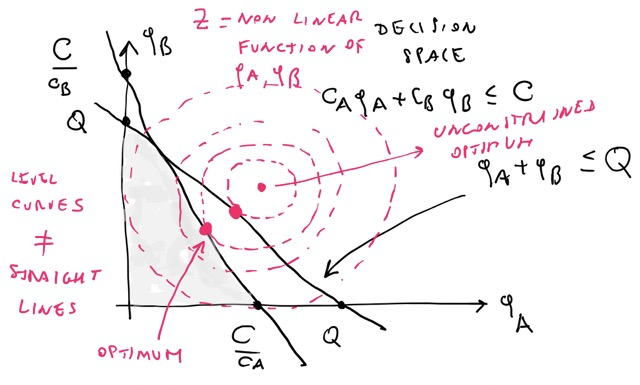
\includegraphics[scale=0.4]{linlivnonlin.jpeg}
\caption{Grafico con linee di livello non lineari} 
\label{linlivnonlin}
\end{figure}


La \hl{funzione obiettivo non e' lineare} dato che $q_A$ e $q_B$ sono al denominatore. Le \hl{curve di livello non sono delle rette} ma saranno concentriche (su ognuna il costo è sempre costante).

Avremo una \hl{soluzione ottima dalla curva di livello tangente all'insieme di ammissibilita'}. Si vado allora a prendere le curve peggiori fino ad arrivare a quella che interseca la regione ottima.


% Algoritmo del simplesso
\subsection{Algoritmo del simplesso}

Ogni problema di ottimizzazione lineare si può \hl{trasformare in forma standard}. Prendiamo un f.o.:

$$\min z = \underline{c}^T \underline{x}$$

e dei vincoli:

\begin{itemize}
	\item $\underline{\underline{A}}\ \underline{x} = \underline{b}$
	\item $\underline{x} \geq 0$
	\item $n > m$
\end{itemize}

con $n$ righe e $m$ colonne delle matrice $\underline{\underline{A}}$.

Utilizziamo l'\hl{operazione di Pivot}, quindi il vincolo:

$$\underline{\underline{A}}\ \underline{x} = \underline{b}$$

sarà:


$$
\left[ {\begin{array}{cccc}
	4 & 1 & 5 & 7 \\
	2 & 3 & 2 & 1 \\
\end{array} } \right]
\left[ {\begin{array}{c}
	x_1 \\
	x_2 \\
	x_3 \\
	x_4 \\
\end{array} } \right]
=
\left[ {\begin{array}{c}
	10 \\
	10 \\
\end{array} } \right]
$$

Il Pivot che ci viene assegnato è:

$$(r, s) = (1, 3)$$

alla quale coordinata corrisponde il valore della prima riga e terza colonna: $5$.

Dai dati \hl{creiamo un sistema di eq lineari}:

$$
\begin{cases} 
    4x_1 + x_2 + 5x_3 + 7x_4 = 10 \\ 
    2x_1 + 3x_2 + 2x_3 + 1x_4 = 10 
\end{cases}
$$

Per eseguire l'operazione di Pivot andremo a far si che \hl{in corrispondenza della colonna di Pivot ($s$) ci sia solo un vettore unitario}:

$$
\left[ {\begin{array}{cccc}
	? & ? & 1 & ? \\
	? & ? & 0 & ? \\
\end{array} } \right]
\left[ {\begin{array}{c}
	x_1 \\
	x_2 \\
	x_3 \\
	x_4 \\
\end{array} } \right]
=
\left[ {\begin{array}{c}
	? \\
	? \\
\end{array} } \right]
$$

Gli steps da seguire sono:

\begin{enumerate}
	\item facciamo \hl{$\frac{r}{a_{rs}}$}, con:
		
		\begin{itemize}
			\item $r$: riga Pivot
			\item $a_{rs} \neq 0$: valore che si trova dal Pivot, nel nostro caso $5$
		\end{itemize}
		
		Diremo quindi che:
		
		$$a_{rj} = \frac{a_{rj}}{a{rs}}\ \ \ \forall\ \ \ j = 1, ..., n+1$$

		$$
		\left[ {\begin{array}{cccc}
			\frac{4}{5} & \frac{1}{4} & 1 & \frac{7}{5} \\
			? & ? & 0 & ? \\
		\end{array} } \right]
		\left[ {\begin{array}{c}
			x_1 \\
			x_2 \\
			x_3 \\
			x_4 \\
		\end{array} } \right]
		=
		\left[ {\begin{array}{c}
			2 \\
			? \\
		\end{array} } \right]
		$$
	
	\item per ogni riga non Pivot $i \neq r$ applichiamo il principio di equivalenza per eq non lineari:
	
		$$\text{riga } i = \text{riga } i + (-a_{is}) * \text{nuova riga } r$$
		
		in questo caso andiamo a sommare $-2$ in modo da avere la configurazione $(1, 3) = 1$ e $(2, 3) = 0$.
		
		Diremo quindi che:
		
		$$a_{ij} = a{ij} + (-a{is})a_{rj}\ \ \ \forall\ \ \ i = 1, ..., m;\ i \neq r$$
		
		\begin{table}[!h]
		    \begin{center}
				\def\arraystretch{2}
		    	\begin{tabular}{| c c c c | c |}
		    	    \hline
		    	    \textbf{col 1} & \textbf{col 2} & \textbf{col 3} & \textbf{col 4} & \textbf{ris} \\\hline
		    	    $\ \ 2$ & $\ \ 3$ & $\ \ 2$ & $\ \ 1$ & $\ 10\ +$ \\
		     		$-\frac{8}{5}$ & $-\frac{2}{5}$ & $-2$ & $-\frac{14}{5}$ & $-4\ =$ \\\hline
		     		$\ \frac{2}{5}$ & $\ \frac{13}{5}$ & $\ \ 0$ & $-\frac{9}{5}$ & $\ \ 6$ \\
					\hline
		    \end{tabular}
		\end{center}
		\end{table}
		
		quindi abbiamo:
		
		$$
		\left[ {\begin{array}{cccc}
			\frac{4}{5} & \frac{1}{4} & 1 & \frac{7}{5} \\
			\frac{2}{5} & \frac{13}{5} & 0 & -\frac{9}{5} \\
		\end{array} } \right]
		\left[ {\begin{array}{c}
			x_1 \\
			x_2 \\
			x_3 \\
			x_4 \\
		\end{array} } \right]
		=
		\left[ {\begin{array}{c}
			2 \\
			6 \\
		\end{array} } \right]
		$$
	
\end{enumerate}


% Tableau
\subsection{Tableau}

Possiamo quindi riscrivere la forma standard con il Tableau con una \hl{forma tabellare} del tipo:

$$ \underline{\underline{\overline{A}}} =
\left[ {\begin{array}{cc}
	\underline{\underline{A}} & \underline{b} \\
	c^T & 0 \\
\end{array} } \right]
$$

dove $m$ righe e $n$ colonne.

I nostri problemi hanno variabili continue dove usando l'algoritmo del simplesso avremo come \hl{forma generale}:

$$\min c_1x_1 + ... + c_n x_n$$

per i vincoli invece:

\begin{itemize}
	\item $a_{11}x_1 + ... + a_{an}x_n = b_1$
	\item \dots
	\item $a_{m1}x_1 + ... + a_{mn}x_n = b_m$
	\item $x_1, ..., x_n \geq 0$
\end{itemize}

\hl{Assumiamo che}:

\begin{enumerate}
	\item $n > m$
	\item $\text{rank}(\underline{A}) = n$
\end{enumerate}

così \hl{non avremo vincoli ridondanti}.

Applichiamo poi la definizione di \hl{insieme di base $B$} (con $\underline{x}_B \in R^m$) ed \hl{insieme non di base $N$} (con $\underline{x}_N \in R^{n-m}$).

quindi avrò che:

$$\underline{x} = (\underline{x}_B, \underline{x}_N)$$

allora:

$$\underline{\underline{A}} = [\underline{\underline{B}} | \underline{\underline{N}}]$$

Se la matrice \hl{$B$ non e' singolare posso ricavare una soluzione} imponendo $$\underline{x}_N:=0$$

Per le \hl{variabili $B$} avremo:

$$\underline{\underline{B}}\ \underline{x}_B = \underline{b}\ \ \ \to\ \ \ \underline{x}_B = \underline{\underline{B}}^{-1}\ \underline{b}$$

sarà anche \hl{ammissibile se $\geq 0$}

Tutto questo grazie al \hl{teorema fondamentale} che dice:

\begin{enumerate}
	\item se un problema ha \textbf{soluzione ammissibile}, allora almeno una \textbf{è di base}.
	\item se \textbf{ammette soluzioni ottime}, c'è n'è almeno \textbf{una di base}
\end{enumerate}


Le soluzioni di base sono quindi più comode dato che sono più piccole in un insieme $R^n$ di soluzioni non ammissibili, ammissibili e ottime.


\begin{figure}[H]
\centering
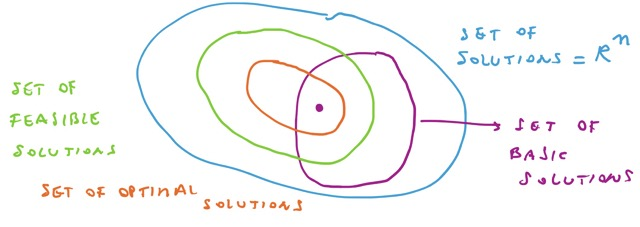
\includegraphics[scale=0.4]{inssol.jpeg}
\caption{Insiemi delle soluzioni} 
\label{inssol}
\end{figure}


Capiamo allora che i \hl{modi per poter scegliere $x_B$} saranno dati dal numero di combinazioni di $n$ elementi di classe $m$:

$$ \binom{n}{m} = \frac{n!}{m!(n-m)!}$$


% Esempio Tableau
\subsection{Esempio Tableau}

Funzione obiettivo:

$$\min z = 2x_1 + 3x_2 + 4x_3 - 5x_4$$

vincoli:

\begin{itemize}
	\item $x_1 - x_2 + x_3 + 2x_4 = 3$
	\item $2x_2 + x_4 = 7$
	\item $x_1 + 2x_3 = 10$
	\item $x_1, x_2, x_3, x_4 \geq 0$
\end{itemize}

Supponiamo: $m = 3$ e $n = 4$.

e scegliamo sull'insieme di tutte le variabili, combinazioni lineari di tanti numeri quante sono le equazioni. Prendiamo per esempio:

\begin{itemize}
	\item $\underline{x}_B = (x_1, x_3, x_4)$
	\item $\underline{x}_N = (x_2)$
\end{itemize}

Andiamo allora a prendere i termini delle variabili e a inserirli in $A$:

$$A =
\left[ {\begin{array}{cccc}
	1 & -1 & 1 & 2\\
	0 & 2 & 0 & 1\\
	1 & 0 & 2 & 0\\
\end{array} } \right]
$$

Dalla f.o. troviamo:

$$c^T = (2, 3, 4, -5)$$

Andremo poi a distribuire a ogni matrice i suoi dati:

$$B =
\left[ {\begin{array}{ccc}
	1 & 1 & 2 \\
	0 & 0 & 1 \\
	1 & 2 & 0 \\
\end{array} } \right]
$$

$$\underline{c}_B = (2, 4, -5)$$

$$N =
\left[ {\begin{array}{c}
	-1 \\
	2 \\
	0 \\
\end{array} } \right]
$$

nel nostro caso c sarà:

$$\underline{c}_N = (3)$$


possiamo allora riscrivere come:

$\min \underline{c}^T_B \underline{x}_B + \underline{c}^T_N \underline{x}_N$


% Forma canonica
\subsection{Forma canonica}

Con le operazioni Pivot \hl{poniamo il problema in forma canonica rispetto a una base}:


$$
\left[ {\begin{array}{ccccc}
	2  & 1  & 4   & -2 & 10\\
	1  & 2  & 4   & 2  & 10\\
	10 & 10 & -2  & 2  & 0 \\
\end{array} } \right]
$$


dove:

\begin{itemize}
	\item \textbf{vincoli} (prime righe):

		\begin{itemize}
			\item[] $2x_1 + x_2 + 4x_3 - 2x_4 = 10$
			\item[] $x_1 + 2x_2 + 4x_3 - 2x_4 = 10$
		\end{itemize}

	\item \textbf{funzione obiettivo} (ultima riga): $$10x_1 + 10x_2 - 2x_3 + 2x_4 + (-z) = 0$$

\end{itemize}

quindi la \hl{funzione obiettivo} è:

$$\min z = 10x_1 + 10x_2 - 2x_3 + 2x_4 + 0$$

e avrà ovviamente tutte le variabili $\geq  0$.


Se effettuo un'\hl{operazione di Pivot} su $(0, 3)$:


$$
\left[ {\begin{array}{ccccc}
	-1 & -0.5 & -2 & 1 & -5\\
	3  &   3  & 8  & 0 & 20\\
	12 &   11 & 2  & 0 & 10\\
\end{array} } \right]
$$

ed un'altra operazione di Pivot su $(1, 1)$:


$$
\left[ {\begin{array}{ccccc}
	-0.5 & 0 & -0.6   & 1 & -1.6\\
	1  	 & 1 & 2.6    & 0 &  6.6\\
	1    & 0 & -27.6  & 0 & -63.3\\
\end{array} } \right]
$$


Il \hl{sistema vincolare e' risolto per $x_2$ e $x_4$} dato che sono quelle \hl{scelte dal Pivot}. Poniamo poi $x_1, x_3 := 0$ ed avremo:

$$x_4 = -1.6,\ x_2 = 6.6$$

quindi avremo una \hl{soluzione base}:

$$\underline{x} = (0, 6.6, 0, -1.6)$$

Questa soluzione è \hl{inammissibile perche' $x_4 \leq 0$} quindi non è Basic Feasible Solution (BFS).

Per esprimere la forma canonica diciamo che gli \hl{indici di colonna delle variabili di $B$ e $N$} sono:

$$I_B = <1, 3>$$
$$I_N= <0, 2>$$

possiamo dire la \hl{posizione delle variabili in base alle equazioni} con:

$$\beta(0) = 3$$
$$\beta(1) = 1$$

\hl{Una forma canonica mi da una soluzione base} andando a porre le \hl{variabili non di base $= 0$} e trovando quelle di base.

Il \hl{valore in basso a destra del Tableau} rappresenta il valore:

$$z = x_1 -27.3x_3 + 63.3$$

dove essendo $x_1$ e $x_3$ non di base:

$$\overline{z} = 63.3$$

quindi rappresenta il \hl{valore della soluzione di base associato a questa forma canonica}.


% Generalizzazione forma canonica
\subsection{Generalizzazione forma canonica}

Generalizzando avrò come \hl{funzione obiettivo}:

$$\min z = \sum_{j \in  I_N} \overline{c}_jx_j + \overline{z}$$

e con \hl{vincoli}:

$$x_{\beta(i)} + \sum_{j \in  I_N} \overline{a}_{ij}x_j = \overline{b}_i\ \ \ \forall\ \ \ i = 0, ..., m - 1$$

con ovviamente $x_j \geq 0, j \in J_N \cup J_B$

L'\hl{equazione di base associata} sarà:

$$x_j := 0\ \ \ \forall\ \ \ j \in J_N$$
$$x_{\beta(i)} = \overline{b}_i \leq \geq 0\ \ \ \forall\ \ \ i = 0, ..., m-1$$

\hl{Pseudocodice} dell'algoritmo del simplesso:

Andremo a:

\begin{enumerate}
	\item trovo la prima \hl{BFS}
	\item in loop faccio:
		\begin{itemize}
			\item un \hl{test di ottimalita'}
			\item se fallisce allora \textbf{sarà migliorabile}
			\item allora mi \textbf{muovo nei dintorni} del suo spazio per migliorare la situazione
		\end{itemize}
	\item se trovo una soluzione di base ammissibile ottima faccio un \hl{analisi per capire se e' unica} o meno
\end{enumerate}


Avremo la \hl{forma generale} quando è \hl{$\leq$ e $\underline{b} \geq 0$}.

Per il \hl{test di ottimalita' in forma canonica}:

$$\min z = \sum_{j \in  I_N} \overline{c}_jx_j + \overline{z}$$

il che significa che per $\underline{x}$ la soluzione ammissibile sarà:

$$z(\underline{x}) = \sum_{j \in  I_N} \overline{c}_jx_j + \overline{z}$$

allora \hl{se $\overline{c}_j \geq 0$ avremo una forma ottimale}, dato che $z(\underline{x}) \geq \overline{z}$

Se \hl{parto dalla soluzione di base ammissibile e prendo una variabile fuori base rendendola positiva}, la funzione obiettivo varia in base alla relazione:

$$z = \sum_{j \in J_N} \overline{c}_j...(slide)$$

cioè \hl{$x_j = 0 \to 1$}

Avremo quindi che la variazione della funzione obiettivo è uguale al coefficiente di posto ridotto $\overline{c}_j$: \hl{$\Delta z = \overline{c}_j$}.

Riusciamo così a \hl{diminuire $z$} il che ci piace perché stiamo minimizzando.

Se il \hl{test di ottimalita' fallisce} perché esiste una variabile di base con coefficiente di costo ridotto negativo potremo avere 2 situazioni:


\begin{figure}[H]
\centering
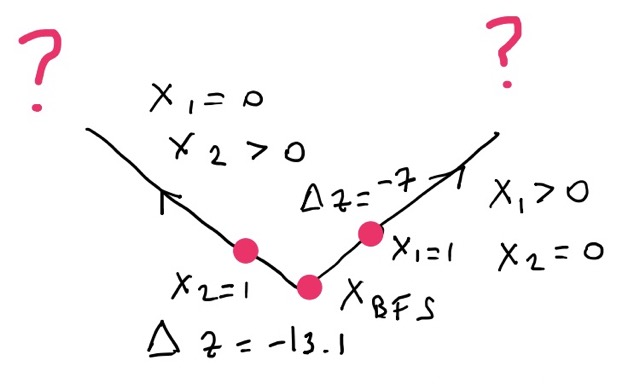
\includegraphics[scale=0.2]{2sol.jpeg}
\caption{Soluzioni per ottimalità} 
\label{2sol}
\end{figure}


Se ho più variabili di base negative allora devo capire \hl{quale delle due devo perturbare}, cioè rendere $> 0$, e la \hl{scegliamo con un "euristica"} che è una scelta algoritmica basata sull'intuizione e info pregresse.

Sceglieremo come variabile, detta variabile entrante, quella con \hl{coefficiente di costo piu' negativo}:

$$x_s = \min_{j \in I_N} \overline{c}_j$$

quindi se $\Delta z = \overline{c}_s x_s$

Se dobbiamo \hl{minimizzare avremo l'interesse e far raggiungere a $x_s$ il valore piu' elevato possibile} dato che ci sarà un miglioramento.

Applichiamo un \hl{vincolo sul massimo valore che $x_s$ puo' raggiungere}:

$$x_s = 0 \to\ > 0$$
$$x_j = 0\ \ \ \forall\ \ \ j \in I_N,\ j \neq s$$

allora avremo:
$$\min z = \overline{c}_s x_s + \overline{z}$$

con vincoli:

\begin{itemize}
	\item $x_{\beta(i)} + \overline{a}_{is}x_s = \overline{b}_i\ \ \ \forall\ \ \ i = 1, ..., m$
	\item $x_j \geq 0\ \ \ \forall\ \ \ j = 1, ..., m$
\end{itemize}

avremo quindi che \hl{$x_s$ cresce fino al non superamento dei vincoli}:

$$x_{\beta(i)} = \overline{b}_i - \overline{a}_{is}x_s \geq 0$$

A questo punto avremo 2 casi possibili:
\begin{enumerate}
	\item avremo:
		$$\overline{a}_{is} \leq 0\ \ \ \forall\ \ \ i = 1, ..., m$$
		allora:
		$$x_{\beta(i)} \geq 0\ \ \ \forall\ \ \ x_s \to +\infty$$
		
		con: $z \to -\infty$
	
	\item avremo:
		$$\exists\ i : \overline{a}_{is} > 0$$

		per calcolare il \hl{massimo valore che $x_s$ puo' assumere} è dato da:

		$$-\overline{a}_{is} x_s \geq -\overline{b}_i$$
		$$\Rightarrow x_s \leq \frac{\overline{b}_i}{\overline{a}_{is}}\ \ \ \forall\ \ \ i = 1, ..., m;\ \overline{a}_{is} > 0$$

		di conseguenza i \hl{valori con $\overline{a}_{is}$ negativo non ci danno problemi dato che $x_{\beta(i)}$ sara' positivo lo stesso} e poi avremo che che:

		$$x_s = \min \frac{\overline{b}_i}{\overline{a}_{is}}\ \ \ \forall\ \ \ i = 1, ..., m;\ \overline{a}_{is} > 0$$


		\begin{figure}[H]
		\centering
		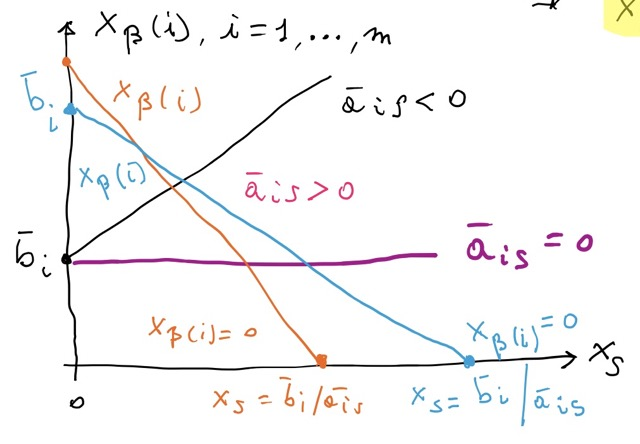
\includegraphics[scale=0.4]{bi.jpeg}
		\caption{Possibilità con i valori di $\overline{a}_{is}$} 
		\label{bi}
		\end{figure}


		Per \hl{$\overline{a}_{is} > 0$} avremo che ad un certo punto \hl{$x_s$ arrivera' a 0}. Ma potrebbe capitare che ci sia \hl{un'altra variabile che diventi 0 prima}, per un valore inferiore di $x_s$.

		Per \hl{esempio} se abbiamo una f.o.:
		$$\min z = -10x_1 - 10x_2 + 0$$

		vincoli:
		\begin{itemize}
			\item $2x_1 + x_2 + x_3 = 10$
			\item $x_1 + 2x_2 + x_4 = 10$
			\item $x_1, x_2, x_3, x_4 \geq 0$\\
		\end{itemize}

		BFS:
		\begin{itemize}
			\item $x_1 = x_2 = 0$
			\item $x_3 = 10$
			\item $x_4 = 10$
			\item $\hat{z} = 0$\\
		\end{itemize}

		\hl{allora}:
		$$x_s = \text{argmin} (-10, -10) = x_1$$

		annullando $x_2$, $x_3$, $x_4$:
		$$x_2 \leq \min (\frac{10}{2}, \frac{10}{1}) = 5$$

		il che significa che $x_s = x_1$, ed abbiamo:
		$$x_3 = 10 - 2x_1 \geq 0$$
		$$x_4 = 10 - x_1 \geq 0$$

		allora abbiamo:


		\begin{figure}[H]
		\centering
		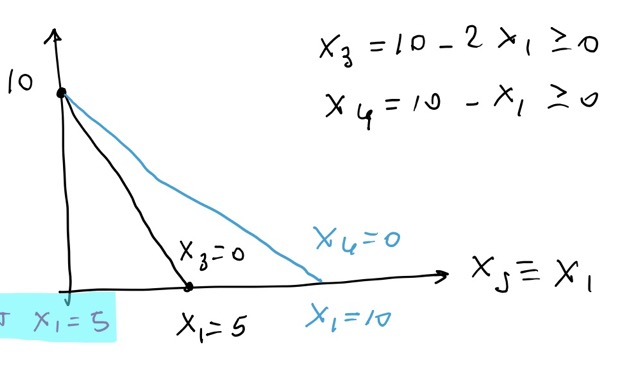
\includegraphics[scale=0.4]{disc.jpeg}
		\caption{Permutazione di $x_1$} 
		\label{disc}
		\end{figure}


		Dopo la nostra perturbazione $x_1 = 0 \to\ 5$ e $x_3 = 10 \to\ 0$, per determinare quale sia la \hl{variabile, detta variabile uscente, che si annulla per prima}:

		$$x_r = \text{argmin} (\frac{10}{2}, \frac{10}{1}) = x_3$$

\end{enumerate}

Lo \hl{pseudocodice} sarà:

\begin{enumerate}
	\item prendere una \hl{BFS}: $x_{BFS}$
	\item in un loop mentre $\exists\ \overline{c}_j \leq 0\ \ \ \forall\ \ \ j \in I_N$:
		\begin{itemize}
			\item $x_s = \text{argmin}_{j \in I_N} \overline{c}_j$
			\item se $\overline{a}_{is} \leq 0\ \ \ \forall\ \ \ i = 1, ..., m$ fa return del problem unbounded
			\item altrimenti $x_2 = \text{argmin} \frac{\overline{b}_i}{\overline{a}_{is}}\ \ \ \forall\ \ \ i = 1, ..., m;\ \overline{a}_{is} > 0$ detta variabile uscente
			\item makePivot(r, s) sennò non posso fare il test di ottimalità una volta reiniziato il loop
		\end{itemize}
\end{enumerate}


% Esercizio forma canonica
\subsection{Esercizio forma canonica}

Funzione obiettivo:

$$\max z = 10x_1 + 10x_2$$

vincoli:

\begin{itemize}
	\item $2x_1 + x_2 \leq 10$
	\item $x_1 + 2x_2 \leq 10$
	\item $x_1, x_2 \geq 0$
\end{itemize}

gradiente:

$$\nabla z =
\left[ {\begin{array}{c}
	10 \\
	10 \\
\end{array} } \right]
$$

grafico:

\begin{figure}[H]
\centering
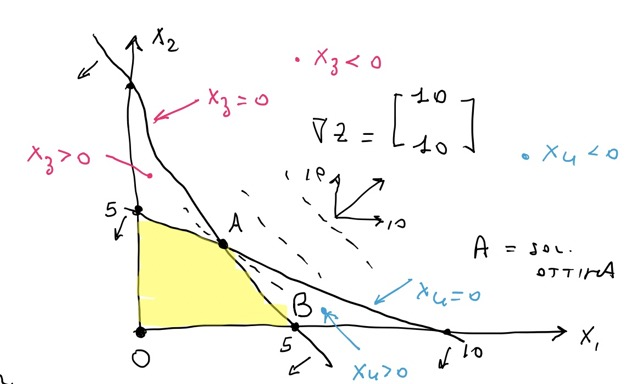
\includegraphics[scale=0.4]{grafescan.jpeg}
\caption{Graficazione dei vincoli} 
\label{grafescan}
\end{figure}

Forma standard:

$$\min z = -10x_1 - 10x_2$$

vincoli:

\begin{itemize}
	\item $2x_1 + x_2 + x_3 = 10$
	\item $x_1 + 2x_2 + x_4 = 10$
	\item $x_1, x_2, x_3, x_4 \geq 0$
\end{itemize}

avremo che:

\begin{itemize}
	\item $A = (3.\overline{3}, 3.\overline{3}, 0, 0)$
	\item $B = (5, 0, 0, > 0)$
	\item $O = (0, 0, > 0, > 0)$
\end{itemize}

dove nei vertici abbiamo \hl{2 variabili $> 0$}. Quindi ad ogni vertice abbiamo una BFS con \hl{cardinalita' $1:M$}.

Tableau:

$$
\left[ {\begin{array}{ccccc}
	2 & 1 & 1 & 0 & 10\\
	1 & 2 & 0 & 1 & 10\\
	-10 & -10 & 0 & 0 & 0\\
\end{array} } \right]
$$

con \hl{variabili} in base $B$ e non in base $N$:

\begin{itemize}
	\item $J_B = <X_3, x_4>$
	\item $J_N = <X_1, x_2>$
\end{itemize}

BFS:

\begin{itemize}
	\item $x_1 = x_2 = 0$
	\item $x_3 = 10$
	\item $x_4 = 10$
	\item $\overline{z} = 0$
\end{itemize}

Il \hl{test di ottimalita' fallisce} e quindi possiamo avere una soluzione migliore. Applico l'\hl{euristica del valore di costo ridotto}. Sceglo a caso $x_s = x_1$.

Prendiamo la \hl{colonna $x_1$ e in base al valore unitario} presente in $x_3$ e $x_4$ allora avremo:
$$\min (\frac{10}{2}, \frac{10}{1}) = 5$$

\hl{non posso avere che $x_3 > 5$} dato che si deve fermare per non diventare negativo, cioè non ammissibile, dato che superiamo in punto $B$.

Allora dato che \hl{$x_3 = 0$ e $x_1$ prende il suo posto} avremo che le \hl{variabili di base cambiano} in:
$$J_B = <x_1, x_4>$$

Dobbiamo allora effettuare un'\hl{operazione di Pivot}:

\begin{itemize}
	\item divido per $2$ la riga 2:
		$$
		\left[ {\begin{array}{ccccc}
			1 & 0.5 & 0.5 & 0 & 5\\
			1 & 2 & 0 & 1 & 10\\
			-10 & -10 & 0 & 0 & 0\\
		\end{array} } \right]
		$$

		\item moltiplico per $-1$ la prima riga e poi sommo alla seconda:
		$$
		\left[ {\begin{array}{ccccc}
			1 & 0.5 & 0.5 & 0 & 5\\
			0 & 1.5 & -0.5 & 1 & 5\\
			-10 & -10 & 0 & 0 & 0\\
		\end{array} } \right]
		$$

		\item moltiplico per $-10$ la prima riga e poi sommo alla terza:
		$$
		\left[ {\begin{array}{ccccc}
			1 & 0.5 & 0.5 & 0 & 5\\
			0 & 1.5 & -0.5 & 1 & 5\\
			0 & -5 & 5 & 0 & 50\\
		\end{array} } \right]
		$$
\end{itemize}

allora abbiamo che la \hl{soluzione di base ammissibile} (BFS) è:

\begin{itemize}
	\item $x_2 = x_3 = 0$
	\item $x_1 = 5$
	\item $x_4 = 5$
	\item $\overline{z} = -50$
\end{itemize}

Nuovamente il test di \hl{ottimalita' fallisce} per la presenza di $-5$, quindi la variabile entrante è $x_s = x_2$ quindi:
$$x_r = \text{argmin} (\frac{5}{0.5}, \frac{5}{1.5}) = x_4$$

il che corrisponde a stare in $B$ dove $x_2 = 0$, quindi ci spostiamo in direzione di $A = (> 0, > 0, 0, 0)$. Avremo allora:
$$J_B = <x_1, x_2>$$

dato che abbiamo \hl{$x_2$ entrante e $x_4$ uscente}.

Il perno del nuovo \hl{Pivot} sarà $1.5$:

$$
\left[ {\begin{array}{ccccc}
	1 & 0 & 0.\overline{6} & -0.\overline{3} & 3.\overline{3}\\
	0 & 1 & -0.\overline{3} & 0.\overline{6} & 3.\overline{3}\\
	0 & 0 & 3.\overline{3} & 3.\overline{3} & 66.\overline{6}\\
\end{array} } \right]
$$

avremo allora: 
\begin{itemize}
	\item $x_3 = x_4 = 0$
	\item $x_1 = 3.\overline{3}$
	\item $x_2 = 3.\overline{3}$
	\item $\overline{z} = -66.\overline{6}$
\end{itemize}

dove abbiamo ottenuto una \hl{soluzione ottima}.


% Soluzioni ottime multiple
\subsection{Soluzioni ottime multiple}

Per individuarle ricordiamo che esiste una soluzione ottima se: 

$$\overline{c_j} \geq 0$$

\hl{esistono soluzioni multiple se esiste $j^{*} \in J_N$} e quindi se ha:

\begin{itemize}
	\item \textbf{coefficienti di costo} ridotti $> 0$
	\item coefficienti delle \textbf{varibiali non di base} sono $> 0$
\end{itemize}

allora \hl{almeno uno sara' $= 0$}. Facendo il solito ragionamento \hl{prendo una variabile $x_{j*} = 0 \to\ > 0$}, allora avrò che:

$$\Delta z = \overline{c}_{j*} x_{j*} = 0$$


% Esempio soluzioni ottime multiple
\subsection{Esempio soluzioni ottime multiple}

Funzione obiettivo:

$$\max z = 20x_1 + 10x_2$$

vincoli:

\begin{itemize}
	\item $2x_1 + x_2 \leq 10$
	\item $x_1 + 2x_2 \leq 10$
	\item $x_1, x_2 \geq 0$
\end{itemize}

gradiente:

$$\nabla z =
\left[ {\begin{array}{c}
	20 \\
	10 \\
\end{array} } \right]
$$

grafico:

\begin{figure}[H]
\centering
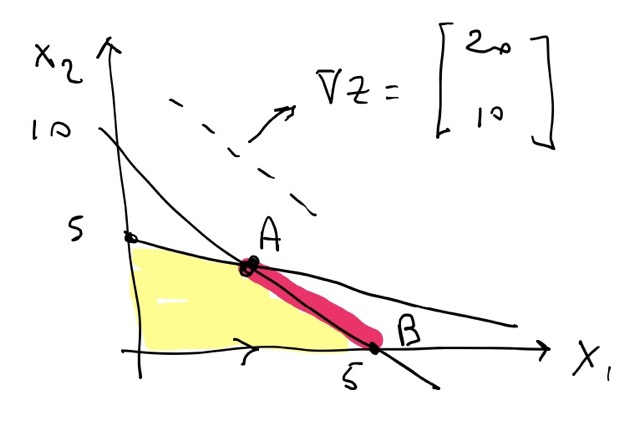
\includegraphics[scale=0.4]{grafsolmult.jpeg}
\caption{Graficazione dei vincoli} 
\label{grafsolmult}
\end{figure}

tableau:

$$
\left[ {\begin{array}{ccccc}
	2 & 1 & 1 & 0 & 10\\
	1 & 2 & 0 & 1 & 10\\
	-20 & -10 & 0 & 0 & 0\\
\end{array} } \right]
$$

BFS:

\begin{itemize}
	\item $x_1 = x_2 = 0$
	\item $x_3 = 10$
	\item $x_4 = 10$
	\item $\overline{z} = 0$
\end{itemize}

Usiamo le operazioni di Pivot:

$$
\left[ {\begin{array}{ccccc}
	1 & 0.5 & 0.5 & 0 & 5\\
	0 & 1.5 & -0.5 & 1 & 5\\
	0 & 0 & 10 & 0 & 100\\
\end{array} } \right]
$$

BFS:

$$B =
\begin{cases} 
    x_2 = x_3 = 0 \\ 
    x_1 = 5 \\
	x_4 = 5 \\
	\overline{z} = -100
\end{cases}
$$

Il \hl{test di ottimalita'} sulle variabili non di base $J_N = <x_2, x_3>$ è OK, \hl{ma non e' una soluzione unica} dato che \hl{abbiamo $0$ per $x_2$} che andrà \hl{perturbata} assegnandole un valore $> 0$. Allora la variazione della funzione obiettivo per una perturbazione è:
$$\overline{c}_{j*}x_{j*}\ \ \ \forall\ \ \ \overline{c}_{j*}=0,\ x_{j*} > 0$$

allora \hl{lungo lo spigolo $\overline{AB}$ avremo un costo minimo}. \hl{Forziamo il Pivot in $x_2$} facendo uscire $x_4$:

$$
\left[ {\begin{array}{ccccc}
	1 & 0 & 0.\overline{6} & -0.\overline{3} & 3.\overline{3}\\
	0 & 1 & -0.\overline{3} & -0.\overline{6} & 3.\overline{3}\\
	0 & 0 & 10 & 0 & 100\\
\end{array} } \right]
$$

BFS:


$$A =
\begin{cases} 
    x_3 = x_4 = 0 \\ 
    x_1 = 3.\overline{3} \\
	x_2 = 3.\overline{3} \\
	\overline{z} = -100
\end{cases}
$$

Abbiamo generato i due punti estremi $A$ e $B$ riuscendo ad avere \hl{infinite soluzioni ottime} dato che ci muoveremo nel segmento $\overline{AB}$. Al massimo potrenno essere:

$$\binom{n}{m}$$ 


% Algoritmo della convergenza
\subsection{Algoritmo della convergenza}

Abbiamo che \hl{se $c_s$ e' la varibiale entrante} allora il costo è dato dalla relazione:

$$\Delta z = \overline{c}_s \min_{i = 1, ..., m}\frac{\overline{b}_i}{\overline{a}_{is}}\ \ \ \forall\ \ \ \overline{a}_{is} > 0$$

con $\overline{c}_s < 0$ e $\min_{i = 1, ..., m}\frac{\overline{b}_i}{\overline{a}_{is}} \geq 0$


L'algoritmo del simplesso \hl{si comporta in modo decrescete} e ad ogni iterazione \hl{genera una nuova BFS}. Se ad ogni iterazione $\Delta z < 0$ vuol dire che avremo come \hl{casi sfavorevoli}:

\begin{itemize}
	\item \hl{$\min < 0$}: l'algoritmo visita tutte le BFS
	\item \hl{$\min = 0$}: uno dei numeratori è nullo
\end{itemize}

Se abbiamo che $x_s = 0$ esisterà un termine noto $\overline{b}_i = 0$ per $\overline{a}_{is} > 0$.

Avremo allora che \hl{se non abbiamo variazioni di $z$} allora \hl{non ci sara' un miglioramento}, dato che l'algoritmo è deterministico genererò la stessa sequenza all'infinito. Questo fenomeno è detto \hl{cycling} e avremo che l'algoritmo non converge.


\begin{figure}[H]
\centering
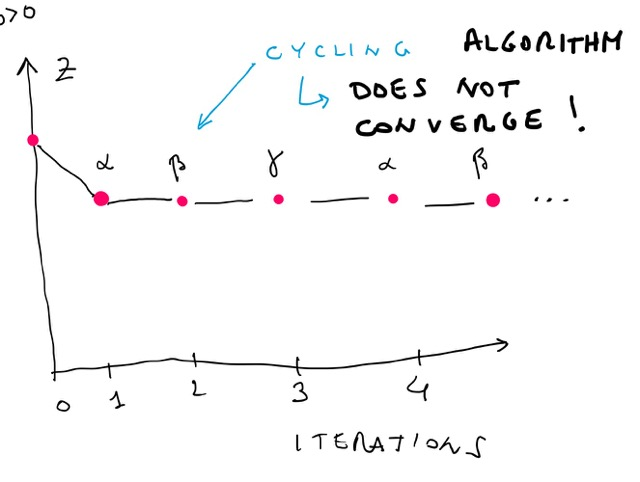
\includegraphics[scale=0.3]{notconv.jpeg}
\caption{Cycling algorithm result} 
\label{notconv}
\end{figure}
	

Potrebbe anche capitare di \hl{avere un miglioramento dopo $n$ iterazioni}.


\begin{figure}[H]
\centering
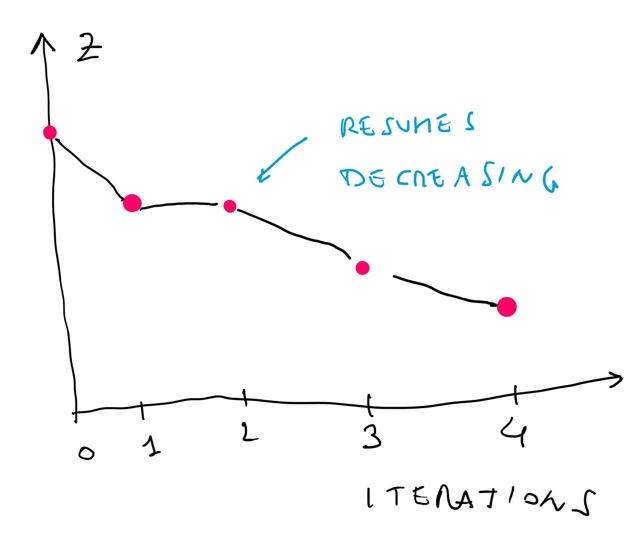
\includegraphics[scale=0.3]{conv.jpeg}
\caption{Not cycling algorithm result} 
\label{conv}
\end{figure}
		
	
% Esempio BFS degenere
\subsection{Esempio BFS degenere}

Funzione obiettivo:
$$\max z = 10x_1 + 10x_2$$

vincoli:

\begin{itemize}
	\item $x_1 - x_2 \leq 0$
	\item $x_2 \leq 1$
	\item $x_1, x_2 \geq 0$
\end{itemize}

grafico:


\begin{figure}[H]
\centering
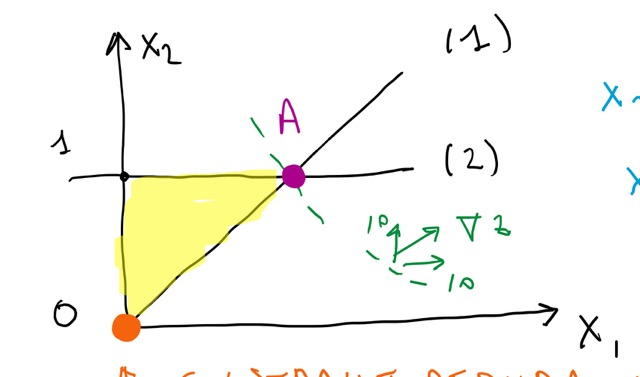
\includegraphics[scale=0.3]{esdegen.jpeg}
\caption{Grafico di un sistema inizialmente degenere} 
\label{esdegen}
\end{figure}

tabelau:

$$
\left[ {\begin{array}{ccccc}
	1 & -1 & 1 & 0 & 0\\
	0 & 1 & 0 & 1 & 1\\
	-10 & -10 & 0 & 0 & 0\\
\end{array} } \right]
$$

dove $\Delta z = 0 * x_1 = 0 * 0 = 0$

Notiamo di avere una variabile in base $= 0$ che sarà detta \hl{variabile degenere}. Dato che abbiamo dei termini negativi, nell'ultima riga, allora \hl{prendiamo quello con numero piu' negativo}, in questo caso anche con l'\hl{indice piu' negativo}$x_s = x_1$, allora:

$$x_r = \text{argmin} (\frac{0}{1}) = x_3$$

con $x_1 \leq \min (\frac{0}{1}) = 0$

Notiamo che abbiamo preso $x_3$ dato che \hl{in corrispondenza del numero piu' grande} abbiamo il valore unitario della colonna di $x_3$. 

Abbiamo un'altra soluzione degenere quindi ci troviamo su un \hl{plateau}. Graficamente abbiamo che $x_1$ rimane 0 nel punto $(0,0)$, avremo allora che nel segmento $\overline{0A}$ ci sarà un \hl{numero ridondante e superfluo di vincoli}. 


$$
\left[ {\begin{array}{ccccc}
	1 & -1 & 1 & 0 & 0\\
	0 & 1 & 0 & 1 & 1\\
	0 & -20 & 10 & 0 & 0\\
\end{array} } \right]
$$


Dove seguendo i motivi detti prima avremo $x_s = x_2$, allora:

$$x_r = \text{argmin}(\frac{1}{1}) = x_4$$

con $x_2 \leq \min(\frac{1}{1}) = 1$

Abbiamo quindi che:
$$\Delta z = -20 * x_2 = -20 * 1 = -20$$

prendendo come perno il valore più alto della colonna $x_2$ avremo un miglioramento:


$$
\left[ {\begin{array}{ccccc}
	1 & 0 & 1 & 1 & 1\\
	0 & 1 & 0 & 1 & 1\\
	0 & 0 & 10 & 20 & 20\\
\end{array} } \right]
$$

quindi con $\Delta z = - 20$.


% Regola dell'anticycling: Bland rule
\subsection{Regola dell'anticycling: Bland rule}

Possiamo \hl{evitare di avere variabili degeneri} usando la Bland Rule. Andremo semplicemente, \hl{a parita' di valore}, a prendere quello con \hl{indice piu' negativo}. Quindi in:


% Variabili artificiali
\subsection{Variabili artificiali}

Iniziamo aggiungendo \hl{ad ogni vicolo} una variabile artificiale:
$$\sum_j a_{ij}x_j + \alpha_i = b_i\ \ \ \forall\ \ \ i = 1, ..., m$$

con $\alpha_i \geq 0\ \ \ \forall\ \ \ i = 1, ..., m$.

Indicato con \hl{$P_a$ il problema artificiale}, la sua \hl{regione ammissibile sara'}:
$$\Omega(P_a) = \{\underline{x} \in R^m : \underline{\underline{A}}\ \underline{x} + \underline{\alpha} = \underline{b},\ \underline{x} \geq 0,\ \underline{\alpha} \geq 0,\ \underline{\alpha} \in R^m\}$$

Invece per il \hl{problema di partenza $P$}, la regione ammissibile è:
$$\Omega(P) = \{\underline{x} \in R^m : \underline{\underline{A}}\ \underline{x} = \underline{b},\ \underline{x} \geq 0\}$$

Avremo allora che:
$$\Omega(P_a) \geq \Omega(P) \Leftrightarrow x \in \Omega(P) \Rightarrow x \in \Omega(P_a)$$

La soluzione \hl{potrebbe comunque non essere ammissibile} per $P$. Allora cerchiamo una soluzione quivalente ma che sia valida sia per $P_a$ che per $P$.

Il problema artificiale (teorema 1) avrebbe come \hl{funzione obiettivo}:
$$\min \rho = \underline{e}^T \underline{\alpha}\ \ \ \forall\ \ \ e = [1, ..., 1]$$

vincoli:

\begin{itemize}
	\item $\underline{\underline{A}}\ \underline{x} + \underline{\alpha} = \underline{b}$
	\item $\underline{x}, \underline{\alpha} \geq 0$
\end{itemize}

Notare che \hl{ammette sempre soluzioni ottime}.

Per il teorema 2 avremo che $P$ è \hl{ammissibile $\Leftrightarrow$ $P_a$ ha $\rho^* = 0$}.

Dati quesi 2 problemi avremo che per:

\begin{enumerate}
	\item \hl{$\rho^* > 0$}: il problema $P$ è \textbf{inammissibile}
	\item \hl{$\rho^* = 0$}: alla soluzione ottima $P_a$ \textbf{corrispone una BFS per $P$}
\end{enumerate}


% Metodo del simplesso in 2 fasi
\subsection{Metodo del simplesso in 2 fasi}

Per prima cosa risolviamo il $P_a$ con il metodo del simplesso. Se \hl{$\rho^* = 0$ usiamo la soluzione ottima di $P_a$} senza le variabili artificiali. Prenderemo poi la \hl{f.o. $z$ come BFS per $P$} e da questa applicare il metodo del simplesso. 


% Costruzione del problema artificiale
\subsection{Costruzione del problema artificiale}

Funzione obiettivo:
$$\min z = \sum_{j = 1}^n c_jx_j$$

vincoli:

\begin{itemize}
	\item $\sum_{j=1}^n a_{ij}x_j \leq b_i\ \ \ \forall\ \ \ i = 1, ..., m_1$
	\item $\sum_{j=1}^n a_{ij}x_j \geq b_i\ \ \ \forall\ \ \ i = m_1+1, ..., m_2$
	\item $\sum_{j=1}^n a_{ij}x_j = b_i\ \ \ \forall\ \ \ i = m_2+1, ..., m$
\end{itemize}

con $x_j \geq 0\ \ \ \forall\ \ \ j = 1, ..., m$.

Forma standard abbiamo che la funzione obiettivo:
$$\min z = \sum_{j = 1}^n c_jx_j$$

vincoli:

\begin{itemize}
	\item $\sum_{j=1}^n a_{ij}x_j + x_{n+i} = b_i\ \ \ \forall\ \ \ i = 1, ..., m_1$
	\item $\sum_{j=1}^n a_{ij}x_j - x_{n+i} = b_i\ \ \ \forall\ \ \ i = m_1+1, ..., m_2$
	\item $\sum_{j=1}^n a_{ij}x_j = b_i\ \ \ \forall\ \ \ i = m_2+1, ..., m$
\end{itemize}

con 

\begin{itemize}
	\item $x_j \geq 0\ \ \ \forall\ \ \ j = 1, ..., n$
	\item $x_{n+i} \geq 0\ \ \ \forall\ \ \ i = 1, ..., m_2$
\end{itemize}

Per fare in modo di avere un problema artificiale con il \hl{minor numero di variabili artificiali} dovremo:

\begin{enumerate}
	\item per \hl{$i = 1, ..., m_1$ NON aggiungiamo variabili artificiali}, dato che abbiamo quelle di slack
	\item per \hl{$i = m_2 + 1, ..., m$ aggiungo una variabile artificiale} per ogni vincolo
	\item per \hl{$i = m_1 + 1, ..., m_2$ aggiungo una $\alpha_0$} in ogni vincolo
\end{enumerate}

Indichiamo un l'\hl{indice $h(m_1+1 \leq h \leq m_2)$} t.c.:
$$h = \text{argmax}_i\{b_i,\ i = m_1+1, ..., m_2\}$$

\hl{Rimpiazziamo ogni vincolo $i \neq h$ con} un vincolo quivalente:
$$\sum (a_{hj} - a_{ij})x_j - x_{n+h} + x_{n+i} = b_n - b_i\ \ \ \forall\ \ \ i = m_1 + 1, ..., m_2,\ i \neq h$$

avremo allora:
$$\sum a_{hj}x_j - x_{n+h} + \alpha_0 = b_n$$
$$\sum a_{ij}x_j - x_{n+i} + \alpha_0 = b_i$$


% Esempio problema artificiale
\subsection{Esempio problema artificiale}

Funzione obiettivo:
$$\min z = 4x_1 + 5x_2$$

vincoli:

\begin{itemize}
	\item $x_1 - x_3 = 6$
	\item $x_2 - x_4 = 4$
	\item $x_1 + 3x_2 = 21$
	\item $x_1, x_2, x_3, x_4 \geq 0$
\end{itemize}

Il problema artificiale è dato dalla funzione obiettivo:
$$\min \rho = \alpha_1 + \alpha_2$$

con vincoli:

\begin{itemize}
	\item $x_1 - x_3 + \alpha_1 = 6$
	\item $x_2 - x_4 + \alpha_1 = 4$
	\item $x_1 + 3x_2 + \alpha_2 = 21$
	\item $x_1, x_2, x_3, x_4, \alpha_1, \alpha_2 \geq 0$
\end{itemize}

Vado ora a \hl{sostituire al vincolo 2 la differenza tra il vincolo 1 e il 2}:
$$x_1 - x_2 - x_3 + x_4 = 2$$

Avremo allora che \hl{$P_a$ e' data da} una funzione obiettivo:
$$\min \rho = \alpha_1 + \alpha_2$$

e dai vincoli:

\begin{itemize}
	\item $x_1 - x_3 + \alpha_1 = 6$
	\item $x_1 - x_2 -x_3 + x_4 = 2$
	\item $x_1 + 3x_2 + \alpha_2 = 21$
	\item $x_1, x_2, x_3, x_4, \alpha_1, \alpha_2 \geq 0$
\end{itemize}

Applichiamo al \hl{prima fase del metodo a 2 fasi}:


$$
\left[ {\begin{array}{ccccccc}
	1 & 0 & -1 & 0 & 1 & 0 & 6\\
	1 & -1 & -1 & 1 & 0 & 0 & 2\\
	1 & 3 & 0 & 0 & 0 & 1 & 21\\
	0 & 0 & 0 & 0 & 1 & 1 & 0\\
\end{array} } \right]
$$

Per poter \hl{ripristinare la forma canonica} dovremo avere i \hl{coefficienti di $\alpha_1,\ \alpha_2 = 0$}. Tramite vari \hl{operazioni di Pivot} arriviamo a non avere più in base $\alpha_1$ e $\alpha_2$. In fine avremo:


$$
\left[ {\begin{array}{ccccc}
	1 & 0 & -1 & 0 & 6\\
	0 & 0 & 0.\overline{3} & 1 & 1\\
	0 & 1 & 0.\overline{3} & 0 & 5\\
	0 & 0 & 2.\overline{3} & 0 & -49\\
\end{array} } \right]
$$

Avremo allora \hl{verificato il criterio di arresto}, perciò avremo una soluzione ottima:
$$x^* = (6, 5, 0, 1),\ z^* = 49$$